\chapter[Fattorizzazione QR e Riflessioni di Householder]{Fattorizzazione QR e Riflessioni di Householder:\\Geometria, Stabilit\`a Numerica e Algoritmi}
\label{chap:fattorizzazione-qr-riflessioni-householder}

Il presente capitolo introduce e analizza in modo costruttivo la \textbf{Fattorizzazione QR}, una delle pietre angolari dell'algebra lineare numerica moderna per il calcolo scientifico, la risoluzione di sistemi lineari sovradeterminati (minimi quadrati) e la computazione spettrale degli autovalori~\cite{golub2013matrix,trefethen1997numerical}. Dopo aver formalizzato il teorema generale di esistenza e la distinzione geometrica tra la decomposizione completa (\textit{Full QR}) e la forma economica (\textit{Thin QR}), viene introdotta la classe dei \textbf{riflettori di Householder} (trasformazioni ortogonali elementari di rango 1). Viene dimostrato il lemma fondamentale di riflessione, affrontando l'impatto critico dell'aritmetica floating-point (cancellazione numerica catastrofica) nella determinazione del riflettore stabile. La trattazione prosegue con la formulazione algoritmica della fattorizzazione mediante sequenze di riflessioni, l'analisi di complessit\`a computazionale, il teorema di unicit\`a e un esempio numerico dettagliato tridimensionale interamente calcolato a mano.

\FloatBarrier
\section{Introduzione alla Fattorizzazione QR e Forme Matriciali}
\label{sec:intro-forme-qr}

\subsection{Teorema di Esistenza della Fattorizzazione QR}

\begin{theorem}[Fattorizzazione QR Completa / Full QR]
\label{thm:qr-esistenza-full}
Per ogni matrice reale rettangolare $A \in \R^{m \times n}$ esistono:
\begin{enumerate}
    \item una matrice ortogonale quadrata $Q \in \R^{m \times m}$, tale che:
    \begin{equation}
        Q^T Q = Q Q^T = I_m;
    \end{equation}
    \item una matrice triangolare superiore estesa $R \in \R^{m \times n}$, tale che:
    \begin{equation}
        R_{i,j} = 0 \quad \text{per ogni } i > j;
    \end{equation}
\end{enumerate}
tali che il loro prodotto riproduca esattamente la matrice di partenza:
\begin{equation}
    A = Q R.
\end{equation}
\end{theorem}

L'importanza computazionale del Teorema~\ref{thm:qr-esistenza-full} risiede nell'eccellente condizionamento delle matrici ortogonali: poich\'e $\|Q\|_2 = 1$ e $\cond_2(Q) = 1$, la moltiplicazione per $Q$ non amplifica gli errori di arrotondamento, preservando la norma euclidea e l'energia dei dati.

\subsection{Geometria e Dimensioni nei Tre Casi Possibili}
A seconda del rapporto dimensionale tra il numero di righe $m$ e il numero di colonne $n$, la fattorizzazione assume forme strutturali differenti:

\begin{figure}[H]
\centering
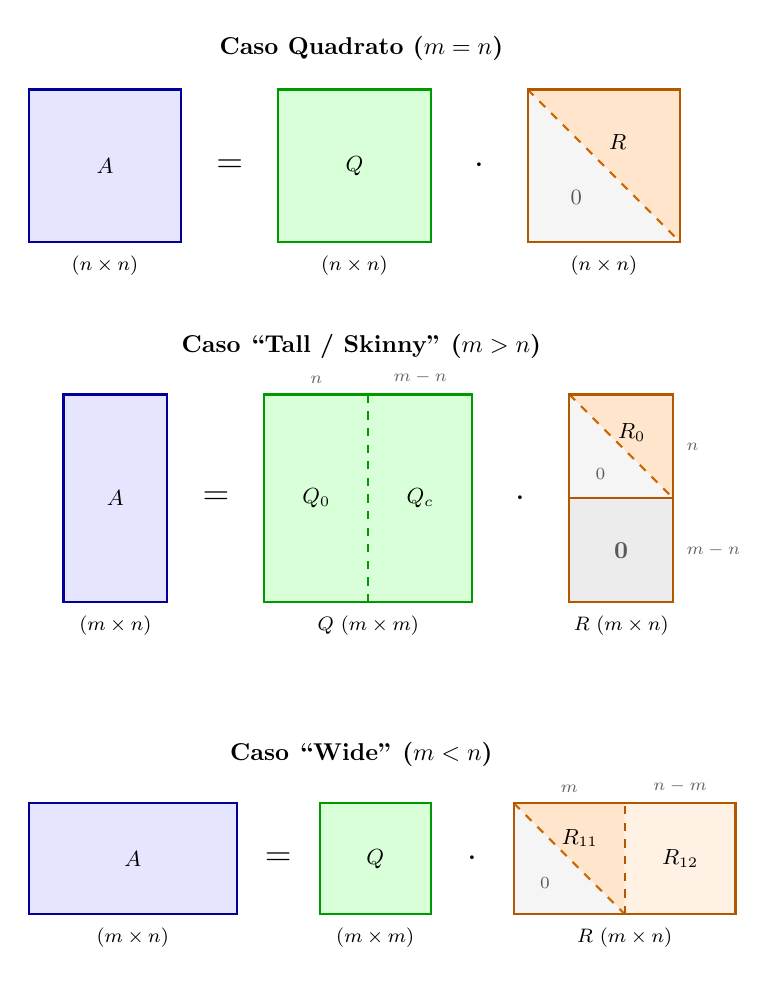
\begin{tikzpicture}[scale=0.88, every node/.style={transform shape}]
    % =========================================================
    % CASO 1: QUADRATO (m = n)
    % =========================================================
    \begin{scope}[yshift=0cm]
        \node[font=\bfseries] at (5.0, 2.8) {Caso Quadrato ($m = n$)};
        
        % Matrice A (n x n)
        \draw[thick, fill=blue!10, draw=blue!60!black] (0.2, 0) rectangle (2.4, 2.2);
        \node[font=\small\bfseries] at (1.3, 1.1) {$A$};
        \node[below=2pt, font=\footnotesize] at (1.3, 0) {$(n \times n)$};
        
        % Simbolo =
        \node[font=\Large\bfseries] at (3.1, 1.1) {$=$};
        
        % Matrice Q (n x n)
        \draw[thick, fill=green!15, draw=green!60!black] (3.8, 0) rectangle (6.0, 2.2);
        \node[font=\small\bfseries] at (4.9, 1.1) {$Q$};
        \node[below=2pt, font=\footnotesize] at (4.9, 0) {$(n \times n)$};
        
        % Simbolo cdot
        \node[font=\Large\bfseries] at (6.7, 1.1) {$\cdot$};
        
        % Matrice R (n x n)
        \fill[orange!20] (7.4, 2.2) -- (9.6, 2.2) -- (9.6, 0) -- cycle;
        \fill[gray!8] (7.4, 2.2) -- (7.4, 0) -- (9.6, 0) -- cycle;
        \draw[thick, dashed, draw=orange!80!black] (7.4, 2.2) -- (9.6, 0);
        \draw[thick, draw=orange!70!black] (7.4, 0) rectangle (9.6, 2.2);
        \node[font=\small\bfseries] at (8.7, 1.45) {$R$};
        \node[font=\small, text=gray!70!black] at (8.1, 0.65) {$0$};
        \node[below=2pt, font=\footnotesize] at (8.5, 0) {$(n \times n)$};
    \end{scope}

    % =========================================================
    % CASO 2: TALL / SKINNY (m > n)
    % =========================================================
    \begin{scope}[yshift=-5.2cm]
        \node[font=\bfseries] at (5.0, 3.7) {Caso ``Tall / Skinny'' ($m > n$)};
        
        % Matrice A (m x n)
        \draw[thick, fill=blue!10, draw=blue!60!black] (0.7, 0) rectangle (2.2, 3.0);
        \node[font=\small\bfseries] at (1.45, 1.5) {$A$};
        \node[below=2pt, font=\footnotesize] at (1.45, 0) {$(m \times n)$};
        
        % Simbolo =
        \node[font=\Large\bfseries] at (2.9, 1.5) {$=$};
        
        % Matrice Q (m x m)
        \draw[thick, fill=green!15, draw=green!60!black] (3.6, 0) rectangle (6.6, 3.0);
        \draw[thick, dashed, draw=green!60!black] (5.1, 0) -- (5.1, 3.0);
        \node[font=\small\bfseries] at (4.35, 1.5) {$Q_0$};
        \node[font=\small\bfseries] at (5.85, 1.5) {$Q_c$};
        \node[above=1pt, font=\scriptsize, text=gray!80!black] at (4.35, 3.0) {$n$};
        \node[above=1pt, font=\scriptsize, text=gray!80!black] at (5.85, 3.0) {$m-n$};
        \node[below=2pt, font=\footnotesize] at (5.1, 0) {$Q \ (m \times m)$};
        
        % Simbolo cdot
        \node[font=\Large\bfseries] at (7.3, 1.5) {$\cdot$};
        
        % Matrice R (m x n)
        % Blocco R_0 (n x n triangolare sup)
        \fill[orange!20] (8.0, 3.0) -- (9.5, 3.0) -- (9.5, 1.5) -- cycle;
        \fill[gray!8] (8.0, 3.0) -- (8.0, 1.5) -- (9.5, 1.5) -- cycle;
        \draw[thick, dashed, draw=orange!80!black] (8.0, 3.0) -- (9.5, 1.5);
        \node[font=\small\bfseries] at (8.9, 2.45) {$R_0$};
        \node[font=\scriptsize, text=gray!70!black] at (8.45, 1.85) {$0$};
        % Blocco 0 inferiore ((m-n) x n)
        \fill[gray!15] (8.0, 0) rectangle (9.5, 1.5);
        \node[font=\bfseries, text=gray!70!black] at (8.75, 0.75) {$\mathbf{0}$};
        % Bordi e divisori
        \draw[thick, draw=orange!70!black] (8.0, 1.5) -- (9.5, 1.5);
        \draw[thick, draw=orange!70!black] (8.0, 0) rectangle (9.5, 3.0);
        \node[right=2pt, font=\scriptsize, text=gray!80!black] at (9.5, 2.25) {$n$};
        \node[right=2pt, font=\scriptsize, text=gray!80!black] at (9.5, 0.75) {$m-n$};
        \node[below=2pt, font=\footnotesize] at (8.75, 0) {$R \ (m \times n)$};
    \end{scope}

    % =========================================================
    % CASO 3: WIDE (m < n)
    % =========================================================
    \begin{scope}[yshift=-9.7cm]
        \node[font=\bfseries] at (5.0, 2.3) {Caso ``Wide'' ($m < n$)};
        
        % Matrice A (m x n)
        \draw[thick, fill=blue!10, draw=blue!60!black] (0.2, 0) rectangle (3.2, 1.6);
        \node[font=\small\bfseries] at (1.7, 0.8) {$A$};
        \node[below=2pt, font=\footnotesize] at (1.7, 0) {$(m \times n)$};
        
        % Simbolo =
        \node[font=\Large\bfseries] at (3.8, 0.8) {$=$};
        
        % Matrice Q (m x m)
        \draw[thick, fill=green!15, draw=green!60!black] (4.4, 0) rectangle (6.0, 1.6);
        \node[font=\small\bfseries] at (5.2, 0.8) {$Q$};
        \node[below=2pt, font=\footnotesize] at (5.2, 0) {$(m \times m)$};
        
        % Simbolo cdot
        \node[font=\Large\bfseries] at (6.6, 0.8) {$\cdot$};
        
        % Matrice R (m x n)
        % Blocco R_11 (m x m triangolare sup)
        \fill[orange!20] (7.2, 1.6) -- (8.8, 1.6) -- (8.8, 0) -- cycle;
        \fill[gray!8] (7.2, 1.6) -- (7.2, 0) -- (8.8, 0) -- cycle;
        \draw[thick, dashed, draw=orange!80!black] (7.2, 1.6) -- (8.8, 0);
        \node[font=\small\bfseries] at (8.15, 1.1) {$R_{11}$};
        \node[font=\scriptsize, text=gray!70!black] at (7.65, 0.45) {$0$};
        % Blocco R_12 (m x (n-m) denso)
        \fill[orange!10] (8.8, 0) rectangle (10.4, 1.6);
        \node[font=\small\bfseries] at (9.6, 0.8) {$R_{12}$};
        % Bordi e divisori
        \draw[thick, dashed, draw=orange!70!black] (8.8, 0) -- (8.8, 1.6);
        \draw[thick, draw=orange!70!black] (7.2, 0) rectangle (10.4, 1.6);
        \node[above=1pt, font=\scriptsize, text=gray!80!black] at (8.0, 1.6) {$m$};
        \node[above=1pt, font=\scriptsize, text=gray!80!black] at (9.6, 1.6) {$n-m$};
        \node[below=2pt, font=\footnotesize] at (8.8, 0) {$R \ (m \times n)$};
    \end{scope}
\end{tikzpicture}
\caption{Struttura dimensionale della decomposizione QR nei tre regimi geometrici ($m = n$, $m > n$ e $m < n$).}
\label{fig:qr-tre-casi}
\end{figure}

\begin{enumerate}
    \item \textbf{Matrice quadrata ($m = n$):}
    $A, Q, R \in \R^{n \times n}$. La matrice $R$ \`e triangolare superiore standard nel senso classico ($R_{i,j} = 0$ per $i > j$).
    \item \textbf{Matrice ``larga'' o orizzontale ($m < n$):}
    $Q \in \R^{m \times m}$ \`e quadrata ortogonale. La matrice $R \in \R^{m \times n}$ ha zeri sotto la diagonale principale delle prime $m$ colonne ($R_{i,j} = 0$ per $i > j$), mentre le restanti $n - m$ colonne sono dense.
    \item \textbf{Matrice ``alta e stretta'' ($m > n$):}
    $Q \in \R^{m \times m}$ \`e quadrata di ordine pieno $m$. La matrice $R \in \R^{m \times n}$ si ripartisce verticalmente in un blocco superiore triangolare $R_0 \in \R^{n \times n}$ e un blocco inferiore di sole righe nulle di dimensione $(m - n) \times n$.
\end{enumerate}

\subsection{Decomposizione QR Economica (Thin / Economy QR)}
Nel contesto comune delle applicazioni di apprendimento automatico e data mining, i dati sono organizzati in matrici ``tall and skinny'' ($m \gg n$, con milioni di osservazioni e decine o centinaia di feature). In tale scenario, memorizzare l'intera matrice ortogonale $Q \in \R^{m \times m}$ richiederebbe $\BigO{m^2}$ elementi di memoria, un costo proibitivo e computazionalmente superfluo.

Partizionando $Q$ per colonne e $R$ per blocchi di righe:
\begin{equation}
    Q = \begin{bmatrix} Q_0 & Q_c \end{bmatrix}, \quad Q_0 \in \R^{m \times n}, \quad Q_c \in \R^{m \times (m-n)},
\end{equation}
\begin{equation}
    R = \begin{bmatrix} R_0 \\ \mathbf{0} \end{bmatrix}, \quad R_0 \in \R^{n \times n}, \quad \mathbf{0} \in \R^{(m-n) \times n}.
\end{equation}
Sviluppando il prodotto a blocchi:
\begin{equation}
    A = Q R = \begin{bmatrix} Q_0 & Q_c \end{bmatrix} \begin{bmatrix} R_0 \\ \mathbf{0} \end{bmatrix} = Q_0 R_0 + Q_c \cdot \mathbf{0} = Q_0 R_0.
\end{equation}

\begin{definition}[Thin / Economy QR]
\label{def:thin-qr}
La fattorizzazione $A = Q_0 R_0$ prende il nome di \textbf{Thin QR} (o \textbf{Economy QR}):
\begin{itemize}
    \item $Q_0 \in \R^{m \times n}$ possiede $n$ colonne ortonormali: $Q_0^T Q_0 = I_n$; tuttavia, in generale $Q_0 Q_0^T \neq I_m$ (non \`e un'isometria globale di $\R^m$, bens\`i il proiettore ortogonale sullo spazio delle colonne di $A$).
    \item $R_0 \in \R^{n \times n}$ \`e una matrice quadrata triangolare superiore.
\end{itemize}
L'impronta di memoria scende da $\BigO{m^2}$ a $\BigO{mn}$, rendendo l'approccio scalabile per grandi basi di dati.
\end{definition}

\FloatBarrier
\section{Applicazioni Fondamentali della Decomposizione QR}
\label{sec:applicazioni-qr}

La decomposizione QR interviene come blocco computazionale primario in svariati ambiti:

\begin{enumerate}
    \item \textbf{Problemi ai Minimi Quadrati Lineari (Ordinary Least Squares):}
    Dato un sistema sovradeterminato $Ax \approx b$ con $A \in \R^{m \times n}$ ($m \ge n$) di rango pieno per colonna, il problema di minimizzazione euclidea:
    \begin{equation}
        \min_{x \in \R^n} \|Ax - b\|_2^2
    \end{equation}
    evita il calcolo delle equazioni normali $A^T A x = A^T b$ (che eleverebbe al quadrato il condizionamento: $\cond_2(A^T A) = \cond_2(A)^2$). Sostituendo la Thin QR $A = Q_0 R_0$, il problema si risolve direttamente sul sistema triangolare superiore:
    \begin{equation}
        R_0 x = Q_0^T b,
    \end{equation}
    risolvibile all'indietro con complessit\`a $\BigO{n^2}$ flops e condizionamento pari a $\cond_2(R_0) = \cond_2(A)$.
    
    \item \textbf{Calcolo Spettrale degli Autovalori (Algoritmo QR):}
    Uno dei dieci algoritmi pi\`u importanti del XX secolo per la diagonalizzazione di matrici generiche o simmetriche genera una successione iterativa di matrici ortogonalmente simili:
    \begin{equation}
        A_k = Q_k R_k \implies A_{k+1} = R_k Q_k = Q_k^T A_k Q_k.
    \end{equation}
    Sotto opportune condizioni, $A_k$ converge asintoticamente alla forma canonica di Schur triangolare superiore, esponendo gli autovalori sulla diagonale.

    \item \textbf{Risoluzione di Sistemi Lineari Quadrati Generici:}
    Se $Ax = b$ con $A \in \R^{n \times n}$ non singolare, $A = QR$ consente di riscrivere il sistema come:
    \begin{equation}
        R x = Q^T b,
    \end{equation}
    sostituendo l'eliminazione gaussiana con pivoting parziale tramite una procedura ortogonalmente stabile.

    \item \textbf{Basi Ortonormali del Sottospazio Immagine:}
    Se $A$ ha rango massimo $n$, le colonne di $Q_0 = [\mathbf{q}_1, \dots, \mathbf{q}_n]$ formano una base ortonormale esatta per lo spazio generato dalle colonne di $A$:
    \begin{equation}
        \operatorname{Im}(A) = \operatorname{span}(Q_0).
    \end{equation}

    \item \textbf{Stabilit\`a Numerica all'Indietro (Backward Stability):}
    A differenza del processo di Gram-Schmidt (che soffre di progressiva perdita di ortogonalit\`a per accumulo di cancellazioni floating-point), l'approccio mediante riflettori di Householder garantisce che i fattori calcolati $\tilde{Q}$ ed $\tilde{R}$ soddisfino esattamente:
    \begin{equation}
        \tilde{Q} \tilde{R} = A + \Delta A, \quad \frac{\|\Delta A\|_2}{\|A\|_2} \le c \cdot \epsilon_{\text{mach}},
    \end{equation}
    garantendo stabilit\`a numerica ottimale.
\end{enumerate}

\FloatBarrier
\section{Matrici Ortogonali Elementari: Problema Introduttivo}
\label{sec:matrici-ortogonali-elementari}

Per formulare costruttivamente un algoritmo numerico in grado di calcolare la fattorizzazione $QR$, studiamo la famiglia delle matrici simmetriche perturbate di rango 1 rispetto all'identit\`a.

\subsection{Formulazione del Problema}
Sia $v \in \R^n$ un vettore di norma unitaria ($\|v\|_2 = 1$, ovvero $v^T v = 1$) e sia $\alpha \in \R$ un parametro scalare reale. Consideriamo la matrice quadrata:
\begin{equation}
    Q = I_n - \alpha v v^T.
    \label{eq:forma-matrice-alfa}
\end{equation}

Affrontiamo le tre questioni analitiche cardine:
\begin{enumerate}
    \item Per quali valori di $\alpha \in \R$ la matrice $Q$ \`e ortogonale?
    \item Per tali valori, qual \`e la forma analitica dell'inversa $Q^{-1}$?
    \item Qual \`e il costo computazionale del prodotto matrice-vettore $Q x$ per un vettore generico $x \in \R^n$?
\end{enumerate}

\subsection{Condizione di Ortogonalit\`a: Derivazione di $\alpha$}
Una matrice quadrata reale $Q$ \`e ortogonale se e solo se $Q Q^T = I$.
Calcoliamo preliminarmente la trasposta di $Q$:
\begin{equation}
    Q^T = (I - \alpha v v^T)^T = I^T - \alpha (v v^T)^T = I - \alpha (v^T)^T v^T = I - \alpha v v^T = Q.
\end{equation}
Dunque, per qualunque valore di $\alpha$, la matrice $Q$ \`e \textbf{simmetrica} ($Q^T = Q$).

Imponendo la condizione di ortogonalit\`a:
\begin{equation}
    Q Q^T = I \iff Q^2 = I \iff (I - \alpha v v^T)(I - \alpha v v^T) = I.
\end{equation}
Sviluppiamo il prodotto sfruttando la propriet\`a distributiva:
\begin{equation}
    (I - \alpha v v^T)(I - \alpha v v^T) = I \cdot I - \alpha v v^T - \alpha v v^T + \alpha^2 (v v^T)(v v^T).
\end{equation}
Sfruttando l'associativit\`a del prodotto matriciale nel termine quadratico:
\begin{equation}
    (v v^T)(v v^T) = v (v^T v) v^T.
\end{equation}
Poich\'e per ipotesi $v$ ha norma unitaria, lo scalare interno $v^T v = \|v\|_2^2 = 1$. L'espressione si riduce pertanto a:
\begin{equation}
    (v v^T)(v v^T) = v (1) v^T = v v^T.
\end{equation}
Sostituendo nuovamente nell'equazione:
\begin{equation}
    I - 2\alpha v v^T + \alpha^2 v v^T = I.
\end{equation}
Sottraendo la matrice identit\`a $I$ da entrambi i membri:
\begin{equation}
    -2\alpha v v^T + \alpha^2 v v^T = \mathbf{0} \iff (\alpha^2 - 2\alpha) v v^T = \mathbf{0}.
\end{equation}
Essendo $v$ un vettore unitario ($v \neq \mathbf{0}$), la matrice esterna diadica $v v^T \neq \mathbf{0}$ non \`e la matrice nulla. L'uguaglianza matriciale sussiste pertanto se e solo se il coefficiente scalare si annulla:
\begin{equation}
    \alpha^2 - 2\alpha = 0 \iff \alpha(\alpha - 2) = 0 \implies \alpha = 0 \quad \text{oppure} \quad \alpha = 2.
\end{equation}

\begin{itemize}
    \item Se $\alpha = 0$, si ottiene $Q = I_n$ (l'identit\`a, banale isometria).
    \item Se $\alpha = 2$, si ottiene la trasformazione non banale:
    \begin{equation}
        Q = I_n - 2 v v^T.
    \end{equation}
    Tale matrice prende il nome di \textbf{riflettore elementare}.
\end{itemize}

\subsection{Calcolo dell'Inversa: La Propriet\`a Involutoria}
Poich\'e la matrice $Q$ \`e contemporaneamente simmetrica ($Q^T = Q$) e ortogonale ($Q^{-1} = Q^T$), per $\alpha = 2$ si deduce immediatamente:
\begin{equation}
    Q^{-1} = Q^T = Q.
\end{equation}
Una matrice che coincide esattamente con la propria inversa, ovvero tale che $Q^2 = I$, viene detta \textbf{involutoria}. Questa propriet\`a possiede un significato geometrico immediato: applicare due volte consecutive una riflessione speculare riporta ogni elemento dello spazio alla sua configurazione iniziale.

\subsection{Costo Computazionale del Prodotto $Q x$}
Dato un generico vettore $x \in \R^n$, dobbiamo valutare il costo operativo per determinare il vettore trasformato $y = Q x = (I - 2 v v^T) x$.

\begin{alertblock}{Principio di Ottimizzazione: Evitare la Materializzazione della Matrice}
Costruire esplicitamente la matrice $Q = I - 2 v v^T$ richiederebbe il calcolo del prodotto diadico $v v^T$ ($\BigO{n^2}$ operazioni) e la memorizzazione di $n^2$ scalari. Inoltre, il successivo prodotto matrice-vettore standard $Q x$ costerebbe ulteriori $2n^2$ flops.
Sfruttando la struttura a rango 1 e l'associativit\`a del prodotto, non materializziamo mai $Q$ come array bidimensionale:
\begin{equation}
    Q x = (I - 2 v v^T) x = x - 2 v (v^T x).
    \label{eq:valutazione-vettore-householder}
\end{equation}
\end{alertblock}

L'algoritmo operativo di calcolo per determinare $y = Q x$ si articola in quattro passaggi sequenziali:
\begin{enumerate}
    \item \textbf{Prodotto scalare interno} $\beta = v^T x = \sum_{i=1}^n v_i x_i$:\\
    Richiede $n$ moltiplicazioni e $n - 1$ addizioni $\implies 2n - 1$ flops ($\BigO{n}$).
    \item \textbf{Moltiplicazione scalare} $\gamma = 2 \beta$:\\
    Richiede $1$ moltiplicazione scalare $\implies 1$ flop ($\BigO{1}$).
    \item \textbf{Scalatura del vettore} $w = \gamma v$:\\
    Richiede $n$ moltiplicazioni tra scalare e componente $\implies n$ flops ($\BigO{n}$).
    \item \textbf{Sottrazione vettoriale} $y = x - w$:\\
    Richiede $n$ sottrazioni componente a componente $\implies n$ flops ($\BigO{n}$).
\end{enumerate}

\paragraph{Complessit\`a complessiva:}
\begin{equation}
    \text{Flops}(Q x) = (2n - 1) + 1 + n + n = 4n \implies \BigO{n}.
\end{equation}
La complessit\`a algoritmica crolla dunque da quadratica $\BigO{n^2}$ a rigorosamente \textbf{lineare} $\BigO{n}$.

\FloatBarrier
\section{Riflettori di Householder e Lemma Fondamentale}
\label{sec:riflettori-householder-lemma}

\subsection{Definizione Generale del Riflettore di Householder}

\begin{definition}[Riflettore di Householder]
\label{def:riflettore-householder}
Sia $v \in \R^n$ un vettore non nullo qualsiasi ($v \neq \mathbf{0}$, non necessariamente normalizzato a norma unitaria). Si definisce \textbf{matrice di Householder} o \textbf{riflettore di Householder} associato al vettore $v$ l'operatore:
\begin{equation}
    H_v = I_n - \frac{2}{\|v\|_2^2} v v^T.
    \label{eq:riflettore-householder-gen}
\end{equation}
\end{definition}

Ponendo $u = \frac{v}{\|v\|_2}$ (versore unitario lungo $v$), si nota che $\frac{2}{\|v\|^2} v v^T = 2 u u^T$, riconducendo la definizione~\eqref{eq:riflettore-householder-gen} alla forma elementare analizzata nella Sezione~\ref{sec:matrici-ortogonali-elementari}. Ne derivano direttamente le propriet\`a fondamentali:
\begin{enumerate}
    \item \textbf{Simmetria:} $H_v^T = H_v$.
    \item \textbf{Ortogonalit\`a e Involutoriet\`a:} $H_v^T H_v = H_v^2 = I_n \implies H_v^{-1} = H_v$.
    \item \textbf{Invarianza per riscalamento:} Per qualsiasi costante reale $c \neq 0$, $H_{c v} = H_v$.
\end{enumerate}

\subsection{Significato Geometrico: Riflessione Rispetto a un Iperpiano}
Consideriamo l'iperpiano vettoriale $(n-1)$-dimensionale $v^\perp \subset \R^n$ ortogonale alla direzione di $v$:
\begin{equation}
    v^\perp = \{z \in \R^n : v^T z = 0\}.
\end{equation}
In virt\`u del teorema di decomposizione ortogonale, ogni vettore $x \in \R^n$ si decompone in modo unico come:
\begin{equation}
    x = x_\parallel + x_\perp,
\end{equation}
dove la componente parallela a $v$ \`e la proiezione ortogonale su $\operatorname{span}(v)$:
\begin{equation}
    x_\parallel = \frac{v^T x}{\|v\|^2} v,
\end{equation}
mentre la componente appartenente all'iperpiano \`e $x_\perp = x - x_\parallel \in v^\perp$.

Applicando l'operatore $H_v$ al vettore $x$:
\begin{equation}
    H_v x = x - \frac{2 v^T x}{\|v\|^2} v = (x_\parallel + x_\perp) - 2 x_\parallel = x_\perp - x_\parallel.
\end{equation}
L'operatore preserva invariata la componente giacente nell'iperpiano ($x_\perp$) e inverte il verso della componente ortogonale ($x_\parallel \mapsto -x_\parallel$). Pertanto, $H_v$ agisce come la \textbf{riflessione ortogonale speculare} rispetto all'iperpiano $v^\perp$.

\begin{figure}[H]
\centering
\begin{tikzpicture}[scale=1.1]
    % Iperpiano v_perp
    \draw[thick, teal!80!black] (-3.5, 0) -- (3.5, 0) node[right, font=\small] {Iperpiano $v^\perp$};
    \fill[teal!5, opacity=0.5] (-3.5, -0.3) rectangle (3.5, 0.3);

    % Vettore normale v
    \draw[-Stealth, thick, red!80!black] (0, 0) -- (0, 2.5) node[above, font=\small] {$v$ (normale all'iperpiano)};

    % Vettore x
    \coordinate (X) at (2.2, 1.8);
    \draw[-Stealth, very thick, blue!80!black] (0, 0) -- (X) node[above right, font=\small] {$x$};

    % Proiezione x_perp e x_parallel
    \coordinate (Xperp) at (2.2, 0);
    \draw[dashed, gray] (X) -- (Xperp);
    \draw[-Stealth, thick, gray!70!black] (0, 0) -- (Xperp) node[below, font=\footnotesize] {$x_\perp$};
    \draw[-Stealth, thick, purple!80!black] (Xperp) -- (X) node[right, midway, font=\footnotesize] {$x_\parallel$};

    % Vettore riflesso H_v(x)
    \coordinate (HX) at (2.2, -1.8);
    \draw[-Stealth, very thick, orange!90!black] (0, 0) -- (HX) node[below right, font=\small] {$H_v x = x_\perp - x_\parallel$};
    \draw[dashed, gray] (HX) -- (Xperp);
    \draw[-Stealth, thick, purple!80!black] (Xperp) -- (HX) node[right, midway, font=\footnotesize] {$-x_\parallel$};

    % Angolo retto
    \draw[thin] (0, 0.3) -- (0.3, 0.3) -- (0.3, 0);
\end{tikzpicture}
\caption{Interpretazione geometrica dell'azione del riflettore di Householder: riflessione speculare rispetto all'iperpiano $v^\perp$.}
\label{fig:householder-riflessione-iperpiano}
\end{figure}

\subsection{Lemma Fondamentale di Riflessione}

\begin{lemma}[Lemma Fondamentale di Riflessione di Householder]
\label{lem:riflessione-fondamentale}
Siano $x, y \in \R^n$ due vettori distinti aventi la medesima norma euclidea, ovvero tali che:
\begin{equation}
    x \neq y \quad \text{e} \quad \|x\|_2 = \|y\|_2.
\end{equation}
Definendo il vettore di Householder come la loro differenza:
\begin{equation}
    v = x - y,
\end{equation}
l'associato riflettore $H_v$ trasforma esattamente il vettore $x$ nel vettore $y$:
\begin{equation}
    H_v x = y.
\end{equation}
\end{lemma}

\begin{proof}
Per definizione del riflettore di Householder applicato al vettore $x$:
\begin{equation}
    H_v x = x - \frac{2}{\|v\|^2} v (v^T x) = x - \frac{2}{\|x - y\|^2} (x - y) \left( (x - y)^T x \right).
    \label{eq:proof-lemma-base}
\end{equation}
Calcoliamo e semplifichiamo separatamente il denominatore scalare e il numeratore scalare:

\paragraph{1. Sviluppo del denominatore $\|x - y\|^2$:}
\begin{equation}
    \|x - y\|^2 = (x - y)^T (x - y) = x^T x - x^T y - y^T x + y^T y.
\end{equation}
Poich\'e il prodotto scalare reale \`e simmetrico ($x^T y = y^T x$) e per ipotesi $\|x\|_2^2 = x^T x = y^T y = \|y\|_2^2$:
\begin{equation}
    \|x - y\|^2 = x^T x - 2 x^T y + x^T x = 2 x^T x - 2 x^T y = 2 (x^T x - x^T y).
    \label{eq:proof-denominatore}
\end{equation}

\paragraph{2. Sviluppo del termine scalare al numeratore $(x - y)^T x$:}
\begin{equation}
    (x - y)^T x = x^T x - y^T x = x^T x - x^T y.
    \label{eq:proof-numeratore}
\end{equation}

\paragraph{3. Sostituzione nell'operatore di riflessione:}
Inserendo le relazioni~\eqref{eq:proof-denominatore} e~\eqref{eq:proof-numeratore} nell'espressione~\eqref{eq:proof-lemma-base}:
\begin{equation}
    H_v x = x - \frac{2}{2 (x^T x - x^T y)} (x - y) (x^T x - x^T y).
\end{equation}
Poich\'e per ipotesi $x \neq y$ e $\|x\| = \|y\|$, per la disuguaglianza di Cauchy-Schwarz con uguaglianza stretta solo per vettori collineari con lo stesso verso, la quantit\`a scalare $x^T x - x^T y = \|x\|^2 - x^T y > 0$ non \`e nulla. Semplificando il fattore scalare comune:
\begin{equation}
    H_v x = x - (x - y) = x - x + y = y.
\end{equation}
La tesi \`e pienamente dimostrata.
\end{proof}

\subsection{Parentesi di Algebra Lineare: Prodotto Interno vs. Prodotto Diadico}
Durante la manipolazione delle forme bilineari matriciali \`e fondamentale distinguere nettamente tra due costrutti:
\begin{itemize}
    \item \textbf{Prodotto scalare (interno):} $x^T y = y^T x \in \R$. \`E un singolo valore numerico, commutativo su $\R$.
    \item \textbf{Prodotto esterno (diadico):} $x y^T \in \R^{n \times n}$. \`E una matrice quadrata di rango 1, e in generale non commuta: $x y^T \neq y x^T = (x y^T)^T$.
\end{itemize}

\begin{example}[Non commutativit\`a del prodotto diadico]
Consideriamo i vettori ortogonali $x = \begin{bmatrix} 2 \\ 0 \end{bmatrix}$ e $y = \begin{bmatrix} 0 \\ 2 \end{bmatrix}$:
\begin{equation}
    x y^T = \begin{bmatrix} 2 \\ 0 \end{bmatrix} \begin{bmatrix} 0 & 2 \end{bmatrix} = \begin{bmatrix} 0 & 4 \\ 0 & 0 \end{bmatrix},
\end{equation}
mentre:
\begin{equation}
    y x^T = \begin{bmatrix} 0 \\ 2 \end{bmatrix} \begin{bmatrix} 2 & 0 \end{bmatrix} = \begin{bmatrix} 0 & 0 \\ 4 & 0 \end{bmatrix} = (x y^T)^T \neq x y^T.
\end{equation}
Al contrario, il loro prodotto scalare coincide e vale $x^T y = y^T x = 0$.
\end{example}

\FloatBarrier
\section{Scelta del Riflettore e Stabilit\`a Numerica}
\label{sec:scelta-riflettore-stabilita}

\subsection{Azzeramento delle Componenti di un Vettore}
Nell'algoritmo di fattorizzazione QR, l'obiettivo operativo consiste nel trasformare un generico vettore colonna $x \in \R^n$ in un multiplo del primo versore canonico $e_1 = [1, 0, \dots, 0]^T$, azzerando tutte le componenti al di sotto della prima:
\begin{equation}
    y = \pm \|x\|_2 e_1 = \begin{bmatrix} \pm \|x\|_2 \\ 0 \\ \vdots \\ 0 \end{bmatrix}.
\end{equation}
Poich\'e $\|\pm \|x\|_2 e_1\|_2 = \|x\|_2$, l'ipotesi di conservazione della norma del Lemma~\ref{lem:riflessione-fondamentale} \`e verificata. Possiamo quindi scegliere come vettore di Householder:
\begin{equation}
    v = x - y = x \mp \|x\|_2 e_1 = \begin{bmatrix} x_1 \mp \|x\|_2 \\ x_2 \\ \vdots \\ x_n \end{bmatrix}.
\end{equation}
In aritmetica teorica esatta, entrambe le scelte di segno garantiscono:
\begin{equation}
    H_v x = \pm \|x\|_2 e_1.
\end{equation}

\subsection{Errore di Cancellazione Catastrofica e Criterio di Stabilit\`a}
Nei calcolatori reali con aritmetica floating-point (standard IEEE 754 a doppia precisione con 53 bit di mantissa e $\epsilon_{\text{mach}} \approx 1.11 \times 10^{-16}$), la sottrazione tra due numeri positivi quasi coincidenti produce una severa perdita di cifre significative, fenomeno noto come \textbf{cancellazione catastrofica}.

Se $x_1 > 0$ e si seleziona il segno meno nella formula, la prima componente del vettore di Householder \`e data da:
\begin{equation}
    v_1 = x_1 - \|x\|_2 = x_1 - \sqrt{x_1^2 + x_2^2 + \dots + x_n^2}.
\end{equation}
Se le componenti al di sotto della diagonale $x_2, \dots, x_n$ sono molto piccole rispetto a $x_1$, si ha $\|x\|_2 \approx x_1$, e la sottrazione $x_1 - \|x\|_2$ elide quasi tutti i bit della mantissa, esponendo il calcolo a un errore relativo gigantesco.

\begin{noteblock}{Regola Aurea di Stabilit\`a per il Riflettore di Householder}
Per evitare qualunque cancellazione numerica, la prima componente di $v$ deve essere espressa sempre come somma di grandezze aventi lo \textbf{stesso segno}:
\begin{itemize}
    \item Se $x_1 \ge 0$, si sceglie il segno positivo:
    \begin{equation}
        v = x + \|x\|_2 e_1 \implies v_1 = x_1 + \|x\|_2,
    \end{equation}
    ovvero una somma di quantit\`a concordi positive ($H_v x = -\|x\|_2 e_1$).
    \item Se $x_1 < 0$, si sceglie il segno negativo:
    \begin{equation}
        v = x - \|x\|_2 e_1 \implies v_1 = x_1 - \|x\|_2 = -(|x_1| + \|x\|_2),
    \end{equation}
    ovvero una somma di quantit\`a concordi negative ($H_v x = +\|x\|_2 e_1$).
\end{itemize}
In forma unificata e compatta:
\begin{equation}
    v = x + \operatorname{sign}(x_1) \|x\|_2 e_1,
    \label{eq:criterio-stabile-householder}
\end{equation}
con la convenzione $\operatorname{sign}(0) = 1$. Il vettore trasformato risulta:
\begin{equation}
    H_v x = -\operatorname{sign}(x_1) \|x\|_2 e_1.
\end{equation}
\end{noteblock}

\subsection{Esperimento Numerico al Calcolatore}
Consideriamo il vettore quadridimensionale con un elemento dominante:
\begin{equation}
    x = \begin{bmatrix} 10^4 \\ 10^{-4} \\ 10^{-4} \\ 10^{-4} \end{bmatrix}.
\end{equation}
La norma euclidea esatta \`e:
\begin{equation}
    \|x\|_2 = \sqrt{10^8 + 3 \cdot 10^{-8}} \approx 10^4 + 1.5 \times 10^{-12}.
\end{equation}
\begin{itemize}
    \item \textbf{Scelta errata ($v = x - \|x\|_2 e_1$):}
    \begin{equation}
        v_1 = 10^4 - (10^4 + 1.5 \times 10^{-12}) = -1.5 \times 10^{-12}.
    \end{equation}
    A causa della perdita di precisione nelle cifre meno significative durante la sottrazione, la determinazione numerica di $v_1$ accumula un errore relativo gravissimo. Applicando l'operatore $H_v$ calcolato al vettore $x$, le componenti dalla seconda alla quarta in $H_v x$ risultano non nulle (dell'ordine di $10^{-4}$ o $10^{-5}$ anzich\'e zero).
    \item \textbf{Scelta corretta conforme alla regola aurea ($v = x + \|x\|_2 e_1$):}
    \begin{equation}
        v_1 = 10^4 + (10^4 + 1.5 \times 10^{-12}) = 2 \cdot 10^4 + 1.5 \times 10^{-12}.
    \end{equation}
    Non si verifica alcuna cancellazione numerica. Il calcolo floating-point restituisce $H_v x$ con zeri esatti (fino alla precisione macchina $\approx 10^{-16}$) per tutte le componenti inferiori.
\end{itemize}

\FloatBarrier
\section{Algoritmo di Fattorizzazione Householder QR}
\label{sec:algoritmo-householder-qr}

L'algoritmo di fattorizzazione QR mediante Householder consiste nell'applicare iterativamente una sequenza di $n - 1$ riflettori a sinistra della matrice $A \in \R^{m \times n}$ ($m \ge n$):
\begin{equation}
    H_{n-1} \cdots H_2 H_1 A = R.
\end{equation}

\begin{figure}[H]
\centering
\begin{tikzpicture}[scale=0.92, every node/.style={transform shape}]
    % =========================================================
    % PASSO 1: A^(1) = H_1 A
    % =========================================================
    \begin{scope}[xshift=0cm]
        \node[font=\bfseries\small] at (1.4, 3.3) {Passo 1: $A^{(1)} = H_1 A$};
        
        % Bordo esterno matrice
        \draw[thick] (0, 0) rectangle (2.8, 2.8);
        
        % Prima riga (modificata dal primo riflettore)
        \fill[orange!25] (0, 2.1) rectangle (2.8, 2.8);
        \draw[thick, draw=orange!60!black] (0, 2.1) -- (2.8, 2.1);
        \node[font=\footnotesize\bfseries, text=orange!90!black] at (0.35, 2.45) {$r_{11}$};
        \node[font=\footnotesize] at (1.05, 2.45) {$*$};
        \node[font=\footnotesize] at (1.75, 2.45) {$*$};
        \node[font=\footnotesize] at (2.45, 2.45) {$*$};
        
        % Prima colonna sotto la diagonale (annullata da H_1)
        \fill[gray!15] (0, 0) rectangle (0.7, 2.1);
        \draw[thick, draw=gray!40] (0.7, 0) -- (0.7, 2.1);
        \node[font=\footnotesize, text=gray!70!black] at (0.35, 1.75) {$0$};
        \node[font=\footnotesize, text=gray!70!black] at (0.35, 1.05) {$0$};
        \node[font=\footnotesize, text=gray!70!black] at (0.35, 0.35) {$0$};
        
        % Sottomatrice attiva tilde{A}^(1)
        \fill[teal!10] (0.7, 0) rectangle (2.8, 2.1);
        \draw[thick, dashed, draw=teal!70!black] (0.7, 0) rectangle (2.8, 2.1);
        \node[font=\small\bfseries, text=teal!80!black] at (1.75, 1.05) {$\tilde{A}^{(1)}$};
        \node[below=2pt, font=\scriptsize, text=gray!80!black] at (1.4, 0) {$(m \times n)$};
    \end{scope}

    % Freccia H_2
    \draw[-Stealth, very thick, blue!70!black] (3.1, 1.4) -- (4.3, 1.4) node[midway, above, font=\footnotesize\bfseries] {$H_2$};

    % =========================================================
    % PASSO 2: A^(2) = H_2 A^(1)
    % =========================================================
    \begin{scope}[xshift=4.6cm]
        \node[font=\bfseries\small] at (1.4, 3.3) {Passo 2: $A^{(2)} = H_2 A^{(1)}$};
        
        % Bordo esterno matrice
        \draw[thick] (0, 0) rectangle (2.8, 2.8);
        
        % Prima riga (invariata)
        \fill[orange!15] (0, 2.1) rectangle (2.8, 2.8);
        \draw[thick, draw=orange!50] (0, 2.1) -- (2.8, 2.1);
        \node[font=\footnotesize\bfseries, text=orange!90!black] at (0.35, 2.45) {$r_{11}$};
        \node[font=\footnotesize] at (1.05, 2.45) {$r_{12}$};
        \node[font=\footnotesize] at (1.75, 2.45) {$*$};
        \node[font=\footnotesize] at (2.45, 2.45) {$*$};
        
        % Seconda riga (modificata da tilde{H}_2)
        \fill[orange!25] (0.7, 1.4) rectangle (2.8, 2.1);
        \draw[thick, draw=orange!60!black] (0.7, 1.4) -- (2.8, 1.4);
        \node[font=\footnotesize\bfseries, text=orange!90!black] at (1.05, 1.75) {$r_{22}$};
        \node[font=\footnotesize] at (1.75, 1.75) {$*$};
        \node[font=\footnotesize] at (2.45, 1.75) {$*$};
        
        % Zeri colonna 1
        \fill[gray!15] (0, 0) rectangle (0.7, 2.1);
        \node[font=\footnotesize, text=gray!70!black] at (0.35, 1.75) {$0$};
        \node[font=\footnotesize, text=gray!70!black] at (0.35, 1.05) {$0$};
        \node[font=\footnotesize, text=gray!70!black] at (0.35, 0.35) {$0$};
        
        % Zeri colonna 2 sotto r_{22}
        \fill[gray!15] (0.7, 0) rectangle (1.4, 1.4);
        \draw[thick, draw=gray!40] (1.4, 0) -- (1.4, 1.4);
        \node[font=\footnotesize, text=gray!70!black] at (1.05, 1.05) {$0$};
        \node[font=\footnotesize, text=gray!70!black] at (1.05, 0.35) {$0$};
        
        % Sottomatrice attiva tilde{A}^(2)
        \fill[teal!10] (1.4, 0) rectangle (2.8, 1.4);
        \draw[thick, dashed, draw=teal!70!black] (1.4, 0) rectangle (2.8, 1.4);
        \node[font=\small\bfseries, text=teal!80!black] at (2.1, 0.7) {$\tilde{A}^{(2)}$};
        \node[below=2pt, font=\scriptsize, text=gray!80!black] at (1.4, 0) {$(m \times n)$};
    \end{scope}

    % Freccia H_3 ...
    \draw[-Stealth, very thick, blue!70!black] (7.7, 1.4) -- (8.9, 1.4) node[midway, above, font=\footnotesize\bfseries] {$H_3 \cdots$};

    % =========================================================
    % FORMA FINALE: R
    % =========================================================
    \begin{scope}[xshift=9.2cm]
        \node[font=\bfseries\small] at (1.4, 3.3) {Forma Finale: $R$};
        
        % Triangolo superiore (valori triangolarizzati)
        \fill[orange!20] (0, 2.8) -- (2.8, 2.8) -- (2.8, 0) -- cycle;
        % Triangolo inferiore (zeri)
        \fill[gray!15] (0, 2.8) -- (0, 0) -- (2.8, 0) -- cycle;
        % Diagonale principale da in alto a sinistra a in basso a destra
        \draw[thick, dashed, draw=orange!80!black] (0, 2.8) -- (2.8, 0);
        % Bordo esterno
        \draw[thick, draw=orange!70!black] (0, 0) rectangle (2.8, 2.8);
        
        % Elementi diagonali ed etichette
        \node[font=\footnotesize\bfseries, text=orange!90!black] at (0.35, 2.45) {$r_{11}$};
        \node[font=\footnotesize\bfseries, text=orange!90!black] at (1.05, 1.75) {$r_{22}$};
        \node[font=\footnotesize\bfseries, text=orange!90!black] at (1.75, 1.05) {$r_{33}$};
        \node[font=\footnotesize\bfseries, text=orange!90!black] at (2.45, 0.35) {$r_{44}$};
        
        \node[font=\Large\bfseries, text=orange!90!black] at (2.0, 2.1) {$R$};
        \node[font=\Large\bfseries, text=gray!70!black] at (0.8, 0.7) {$\mathbf{0}$};
        \node[below=2pt, font=\scriptsize, text=gray!80!black] at (1.4, 0) {Triangolare sup.};
    \end{scope}
\end{tikzpicture}
\caption{Progressione iterativa dell'annullamento sotto-diagonale tramite l'algoritmo di Householder QR.}
\label{fig:householder-iterazioni}
\end{figure}

\subsection{Procedura Dettagliata Passo-Passo}

\paragraph{Passo 1:}
Si considera la prima colonna della matrice $A$, indicata con $a_1 = A_{:, 1} \in \R^m$.
\begin{enumerate}
    \item Si costruisce il vettore di Householder stabile:
    \begin{equation}
        v_1 = a_1 + \operatorname{sign}((a_1)_1) \|a_1\|_2 e_1 \in \R^m.
    \end{equation}
    \item Si forma il riflettore di dimensione piena $H_1 = I_m - \frac{2}{\|v_1\|^2} v_1 v_1^T$.
    \item Si applica la riflessione a tutte le colonne di $A$:
    \begin{equation}
        A^{(1)} = H_1 A = \begin{bmatrix}
        \mp \|a_1\|_2 & * & \cdots & * \\
        0 & * & \cdots & * \\
        \vdots & \vdots & \ddots & \vdots \\
        0 & * & \cdots & *
        \end{bmatrix}.
    \end{equation}
\end{enumerate}

\paragraph{Passo 2:}
Per azzerare gli elementi della seconda colonna senza distruggere gli zeri appena creati nella prima, si isola la sottomatrice attiva di dimensione $(m-1) \times (n-1)$ che esclude la prima riga e la prima colonna.
Sia $\tilde{a}_2 \in \R^{m-1}$ la prima colonna di tale sottomatrice (ovvero $A^{(1)}_{2:m, 2}$).
\begin{enumerate}
    \item Si definisce il vettore di Householder ridotto:
    \begin{equation}
        v_2 = \tilde{a}_2 + \operatorname{sign}((\tilde{a}_2)_1) \|\tilde{a}_2\|_2 e_1 \in \R^{m-1}.
    \end{equation}
    \item Si costruisce il riflettore ridotto $\hat{H}_2 \in \R^{(m-1) \times (m-1)}$:
    \begin{equation}
        \hat{H}_2 = I_{m-1} - \frac{2}{\|v_2\|^2} v_2 v_2^T.
    \end{equation}
    \item Si estende $\hat{H}_2$ all'ordine pieno $m \times m$ tramite immersione a blocchi diagonali:
    \begin{equation}
        H_2 = \begin{bmatrix} 1 & \mathbf{0}^T \\ \mathbf{0} & \hat{H}_2 \end{bmatrix} \in \R^{m \times m}.
    \end{equation}
    L'azione a blocchi preserva intatta la prima riga e la prima colonna:
    \begin{equation}
        A^{(2)} = H_2 A^{(1)} = \begin{bmatrix} 1 & \mathbf{0}^T \\ \mathbf{0} & \hat{H}_2 \end{bmatrix} \begin{bmatrix} A^{(1)}_{1,1} & A^{(1)}_{1, 2:n} \\ \mathbf{0} & A^{(1)}_{2:m, 2:n} \end{bmatrix} = \begin{bmatrix} A^{(1)}_{1,1} & A^{(1)}_{1, 2:n} \\ \mathbf{0} & \hat{H}_2 A^{(1)}_{2:m, 2:n} \end{bmatrix}.
    \end{equation}
\end{enumerate}

\paragraph{Passo $k$ generico ($k = 1, \dots, n-1$ per $m = n$ oppure $k = 1, \dots, n$ per $m > n$):}
Al passo $k$-esimo, la riflessione opera esclusivamente sulla sottomatrice $(m - k + 1) \times (n - k + 1)$ d'angolo inferiore destro:
\begin{equation}
    \hat{H}_k = I_{m-k+1} - \frac{2}{\|v_k\|^2} v_k v_k^T, \qquad H_k = \begin{bmatrix} I_{k-1} & \mathbf{0} \\ \mathbf{0} & \hat{H}_k \end{bmatrix}.
\end{equation}

Al termine degli $n-1$ passi (o $n$ passi se $m > n$), la matrice risultante \`e esattamente triangolare superiore:
\begin{equation}
    R = H_{n-1} \cdots H_2 H_1 A.
\end{equation}
Moltiplicando a sinistra per le matrici inverse (che coincidono con le trasposte e con le matrici stesse $H_k^{-1} = H_k$):
\begin{equation}
    A = Q R, \quad \text{con } Q = H_1 H_2 \cdots H_{n-1}.
\end{equation}
Poich\'e ogni $H_k$ \`e ortogonale e il prodotto di matrici ortogonali \`e una matrice ortogonale, $Q$ \`e rigorosamente ortogonale.

\FloatBarrier
\section{Complessit\`a Computazionale e Propriet\`a di Unicit\`a}
\label{sec:complessita-unicita-qr}

\subsection{Analisi della Complessit\`a Computazionale}
Durante l'esecuzione dell'algoritmo, l'aggiornamento della sottomatrice attiva al passo $k$ viene effettuato applicando la formula lineare~\eqref{eq:valutazione-vettore-householder} a ciascuna delle colonne rimanenti, senza mai formare esplicitamente le matrici $\hat{H}_k$:
\begin{equation}
    \hat{H}_k B = B - \frac{2}{\|v_k\|^2} v_k (v_k^T B).
\end{equation}
Valutando il numero di operazioni in virgola mobile per una matrice quadrata $A \in \R^{n \times n}$:
\begin{itemize}
    \item Al passo $k$, il calcolo del vettore $v_k \in \R^{n-k+1}$ costa $\approx 3(n-k)$ flops.
    \item L'applicazione di $\hat{H}_k$ alle restanti $n - k$ colonne costa $4(n-k)$ flops per colonna, per un totale di $4(n-k)^2$ flops.
\end{itemize}
Sommando su tutti gli $n-1$ passi:
\begin{equation}
    \text{Flops}(R) \approx \sum_{k=1}^{n-1} 4(n-k)^2 \approx 4 \int_0^n x^2 \, dx = \frac{4}{3} n^3 \ \text{flops}.
\end{equation}
Se \`e richiesta anche l'accumulazione esplicita della matrice ortogonale $Q = H_1 \cdots H_{n-1}$, applicando i riflettori all'indietro a partire dall'identit\`a, il costo aggiuntivo \`e pari a ulteriori $\frac{4}{3} n^3$ flops (per un totale di $\approx \frac{8}{3} n^3$ flops).

Per una matrice rettangolare generica $A \in \R^{m \times n}$ con $m \ge n$:
\begin{equation}
    \text{Flops}(R) \approx 2 m n^2 - \frac{2}{3} n^3.
\end{equation}
Nel caso $m \gg n$, il costo \`e asintoticamente pari a $\approx 2 m n^2$ flops.

\subsection{Propriet\`a di Unicit\`a della Fattorizzazione QR}
In generale, la fattorizzazione $A = QR$ \textbf{non \`e unica}. 
Infatti, se $D = \diag(\pm 1, \pm 1, \dots, \pm 1) \in \R^{n \times n}$ \`e una matrice diagonale di segnatura (con soli $+1$ e $-1$ sulla diagonale), allora $D$ \`e ortogonale e simmetrica ($D = D^T = D^{-1}$), e possiamo inserire $D D = I$:
\begin{equation}
    A = Q R = (Q D) (D R) = \tilde{Q} \tilde{R}.
\end{equation}
La matrice $\tilde{Q} = Q D$ ha ancora colonne ortonormali (poich\'e scalare una colonna per $-1$ non ne altera la norma n\'e l'ortogonalit\`a rispetto alle altre), mentre $\tilde{R} = D R$ rimane triangolare superiore (con le righe moltiplicate per $\pm 1$).

Tuttavia, l'ambiguit\`a sui segni pu\`o essere rimossa vincolando gli elementi diagonali di $R$:

\begin{theorem}[Teorema di Unicit\`a Condizionata della Fattorizzazione Thin QR]
\label{thm:qr-unicita-condizionata}
Sia $A \in \R^{m \times n}$ con $m \ge n$ una matrice avente rango massimo per colonna ($\rank(A) = n$).
Se si impone la condizione che tutti gli elementi sulla diagonale principale di $R_0$ siano strettamente positivi:
\begin{equation}
    (R_0)_{i,i} > 0 \quad \text{per ogni } i = 1, \dots, n,
\end{equation}
allora la fattorizzazione Thin QR $A = Q_0 R_0$ \`e \textbf{strettamente unica}.
\end{theorem}

\begin{proof}[Traccia della dimostrazione]
Supponiamo esistano due fattorizzazioni Thin QR con elementi diagonali strettamente positivi: $A = Q_1 R_1 = Q_2 R_2$.
Calcolando la matrice grammaticale $A^T A$:
\begin{equation}
    A^T A = (Q_1 R_1)^T (Q_1 R_1) = R_1^T (Q_1^T Q_1) R_1 = R_1^T I_n R_1 = R_1^T R_1.
\end{equation}
Analogamente, $A^T A = R_2^T R_2$. 
Poich\'e $\rank(A) = n$, la matrice simmetrica $A^T A \in \R^{n \times n}$ \`e strettamente definita positiva (SPD). Per il teorema di unicit\`a della \textbf{Fattorizzazione di Cholesky} ($M = L L^T$), esiste un'unica matrice triangolare inferiore con diagonale positiva tale che $M = L L^T$.
Identificando $L = R_1^T = R_2^T$, si deduce immediatamente $R_1 = R_2$.
Essendo $R_1$ non singolare (poich\'e ha elementi diagonali strettamente positivi), moltiplicando a destra per $R_1^{-1}$:
\begin{equation}
    Q_1 = A R_1^{-1} = A R_2^{-1} = Q_2.
\end{equation}
Dunque $Q_1 = Q_2$ e $R_1 = R_2$, confermando l'unicit\`a assoluta.
\end{proof}

\FloatBarrier
\section[Esempio Numerico Dettagliato (3x3)]{Esempio Numerico Dettagliato (\texorpdfstring{$3 \times 3$}{3x3})}
\label{sec:esempio-numerico-3x3}

\begin{example}[Fattorizzazione Householder QR Completa di una Matrice $3 \times 3$]
Consideriamo la matrice reale:
\begin{equation}
    A = \begin{bmatrix} 
    4 & -5 & -4 \\ 
    3 & 0 & 2 \\ 
    0 & 4 & -3 
    \end{bmatrix}.
\end{equation}
Determiniamo la fattorizzazione $A = QR$ calcolando esplicitamente tutti i riflettori e verificando ogni passaggio.

\paragraph{Passo 1: Azzeramento della prima colonna}
\begin{enumerate}
    \item \textbf{Estrazione della prima colonna:}
    \begin{equation}
        a_1 = \begin{bmatrix} 4 \\ 3 \\ 0 \end{bmatrix}.
    \end{equation}
    \item \textbf{Calcolo della norma euclidea:}
    \begin{equation}
        \|a_1\|_2 = \sqrt{4^2 + 3^2 + 0^2} = \sqrt{16 + 9 + 0} = \sqrt{25} = 5.
    \end{equation}
    \item \textbf{Costruzione del vettore di Householder $v_1$:}
    Poich\'e $(a_1)_1 = 4 > 0$, per scongiurare la cancellazione numerica adottiamo il segno $+$, conformemente alla formula~\eqref{eq:criterio-stabile-householder}:
    \begin{equation}
        v_1 = a_1 + \|a_1\|_2 e_1 = \begin{bmatrix} 4 \\ 3 \\ 0 \end{bmatrix} + \begin{bmatrix} 5 \\ 0 \\ 0 \end{bmatrix} = \begin{bmatrix} 9 \\ 3 \\ 0 \end{bmatrix}.
    \end{equation}
    \item \textbf{Calcolo della norma quadra di $v_1$:}
    \begin{equation}
        \|v_1\|_2^2 = 9^2 + 3^2 + 0^2 = 81 + 9 + 0 = 90.
    \end{equation}
    \item \textbf{Costruzione della matrice di Householder $H_1$:}
    \begin{equation}
        H_1 = I_3 - \frac{2}{\|v_1\|^2} v_1 v_1^T = I_3 - \frac{2}{90} \begin{bmatrix} 9 \\ 3 \\ 0 \end{bmatrix} \begin{bmatrix} 9 & 3 & 0 \end{bmatrix}.
    \end{equation}
    Sviluppiamo il prodotto diadico:
    \begin{equation}
        \frac{2}{90} v_1 v_1^T = \frac{1}{45} \begin{bmatrix} 81 & 27 & 0 \\ 27 & 9 & 0 \\ 0 & 0 & 0 \end{bmatrix} = \begin{bmatrix} 9/5 & 3/5 & 0 \\ 3/5 & 1/5 & 0 \\ 0 & 0 & 0 \end{bmatrix}.
    \end{equation}
    Sottraendo dall'identit\`a $I_3$:
    \begin{equation}
        H_1 = \begin{bmatrix} 1 & 0 & 0 \\ 0 & 1 & 0 \\ 0 & 0 & 1 \end{bmatrix} - \begin{bmatrix} 9/5 & 3/5 & 0 \\ 3/5 & 1/5 & 0 \\ 0 & 0 & 0 \end{bmatrix} = \begin{bmatrix} -4/5 & -3/5 & 0 \\ -3/5 & 4/5 & 0 \\ 0 & 0 & 1 \end{bmatrix}.
    \end{equation}
    \item \textbf{Calcolo del prodotto $A^{(1)} = H_1 A$:}
    \begin{itemize}
        \item \textit{Prima colonna:} Per costruzione ortogonale:
        \begin{equation}
            H_1 \begin{bmatrix} 4 \\ 3 \\ 0 \end{bmatrix} = \begin{bmatrix} -\|a_1\|_2 \\ 0 \\ 0 \end{bmatrix} = \begin{bmatrix} -5 \\ 0 \\ 0 \end{bmatrix}.
        \end{equation}
        Verifica algebrica diretta:
        \begin{align*}
            (-4/5)(4) + (-3/5)(3) &= -\frac{16+9}{5} = -5, \\
            (-3/5)(4) + (4/5)(3) &= -\frac{12}{5} + \frac{12}{5} = 0.
        \end{align*}
        \item \textit{Seconda colonna:}
        \begin{equation}
            H_1 \begin{bmatrix} -5 \\ 0 \\ 4 \end{bmatrix} = \begin{bmatrix} (-4/5)(-5) + (-3/5)(0) \\ (-3/5)(-5) + (4/5)(0) \\ 1(4) \end{bmatrix} = \begin{bmatrix} 4 \\ 3 \\ 4 \end{bmatrix}.
        \end{equation}
        \item \textit{Terza colonna:}
        \begin{equation}
            H_1 \begin{bmatrix} -4 \\ 2 \\ -3 \end{bmatrix} = \begin{bmatrix} (-4/5)(-4) + (-3/5)(2) \\ (-3/5)(-4) + (4/5)(2) \\ 1(-3) \end{bmatrix} = \begin{bmatrix} 16/5 - 6/5 \\ 12/5 + 8/5 \\ -3 \end{bmatrix} = \begin{bmatrix} 2 \\ 4 \\ -3 \end{bmatrix}.
        \end{equation}
    \end{itemize}
    La matrice aggiornata al termine del Passo 1 risulta:
    \begin{equation}
        A^{(1)} = H_1 A = \begin{bmatrix} 
        -5 & 4 & 2 \\ 
        0 & 3 & 4 \\ 
        0 & 4 & -3 
        \end{bmatrix}.
    \end{equation}
\end{enumerate}

\paragraph{Passo 2: Azzeramento della seconda colonna}
\begin{enumerate}
    \item \textbf{Isolamento della sottomatrice $2 \times 2$ attiva:}
    Consideriamo le righe 2--3 e le colonne 2--3 di $A^{(1)}$:
    \begin{equation}
        \begin{bmatrix} 3 & 4 \\ 4 & -3 \end{bmatrix}.
    \end{equation}
    Il vettore da azzerare al di sotto della diagonale \`e:
    \begin{equation}
        \tilde{a}_2 = \begin{bmatrix} 3 \\ 4 \end{bmatrix}.
    \end{equation}
    \item \textbf{Calcolo della norma euclidea:}
    \begin{equation}
        \|\tilde{a}_2\|_2 = \sqrt{3^2 + 4^2} = \sqrt{9 + 16} = \sqrt{25} = 5.
    \end{equation}
    \item \textbf{Costruzione del vettore di Householder $v_2$:}
    Essendo $(\tilde{a}_2)_1 = 3 > 0$, scegliamo il segno $+$:
    \begin{equation}
        v_2 = \tilde{a}_2 + \|\tilde{a}_2\|_2 e_1 = \begin{bmatrix} 3 \\ 4 \end{bmatrix} + \begin{bmatrix} 5 \\ 0 \end{bmatrix} = \begin{bmatrix} 8 \\ 4 \end{bmatrix}.
    \end{equation}
    \item \textbf{Calcolo della norma quadra di $v_2$:}
    \begin{equation}
        \|v_2\|_2^2 = 8^2 + 4^2 = 64 + 16 = 80.
    \end{equation}
    \item \textbf{Costruzione del riflettore ridotto $\hat{H}_2 \in \R^{2 \times 2}$:}
    \begin{align}
        \hat{H}_2 &= I_2 - \frac{2}{\|v_2\|^2} v_2 v_2^T = I_2 - \frac{2}{80} \begin{bmatrix} 8 \\ 4 \end{bmatrix} \begin{bmatrix} 8 & 4 \end{bmatrix} \nonumber\\
        &= I_2 - \frac{1}{40} \begin{bmatrix} 64 & 32 \\ 32 & 16 \end{bmatrix} = \begin{bmatrix} 1 & 0 \\ 0 & 1 \end{bmatrix} - \begin{bmatrix} 8/5 & 4/5 \\ 4/5 & 2/5 \end{bmatrix} \nonumber\\
        &= \begin{bmatrix} -3/5 & -4/5 \\ -4/5 & 3/5 \end{bmatrix}.
    \end{align}
    \item \textbf{Estensione per immersione ad ordine pieno $H_2 \in \R^{3 \times 3}$:}
    \begin{equation}
        H_2 = \begin{bmatrix} 
        1 & 0 & 0 \\ 
        0 & -3/5 & -4/5 \\ 
        0 & -4/5 & 3/5 
        \end{bmatrix}.
    \end{equation}
    \item \textbf{Calcolo della matrice triangolare finale $R = H_2 A^{(1)}$:}
    \begin{itemize}
        \item La prima riga e la prima colonna restano invariate:
        \begin{equation}
            R_{1, :} = \begin{bmatrix} -5 & 4 & 2 \end{bmatrix}, \qquad R_{:, 1} = \begin{bmatrix} -5 \\ 0 \\ 0 \end{bmatrix}.
        \end{equation}
        \item La seconda colonna (righe 2--3) diventa per costruzione:
        \begin{equation}
            \hat{H}_2 \begin{bmatrix} 3 \\ 4 \end{bmatrix} = \begin{bmatrix} -\|\tilde{a}_2\|_2 \\ 0 \end{bmatrix} = \begin{bmatrix} -5 \\ 0 \end{bmatrix}.
        \end{equation}
        \item La terza colonna (righe 2--3) si ricava dal prodotto:
        \begin{align}
            \hat{H}_2 \begin{bmatrix} 4 \\ -3 \end{bmatrix} &= \begin{bmatrix} (-3/5)(4) + (-4/5)(-3) \\ (-4/5)(4) + (3/5)(-3) \end{bmatrix} \nonumber\\
            &= \begin{bmatrix} -12/5 + 12/5 \\ -16/5 - 9/5 \end{bmatrix} = \begin{bmatrix} 0 \\ -5 \end{bmatrix}.
        \end{align}
    \end{itemize}
    Otteniamo la matrice triangolare superiore $R$:
    \begin{equation}
        R = \begin{bmatrix} 
        -5 & 4 & 2 \\ 
        0 & -5 & 0 \\ 
        0 & 0 & -5 
        \end{bmatrix}.
    \end{equation}
    \item \textbf{Calcolo della matrice ortogonale $Q = H_1 H_2$:}
    \begin{align}
        Q &= \begin{bmatrix} 
        -4/5 & -3/5 & 0 \\ 
        -3/5 & 4/5 & 0 \\ 
        0 & 0 & 1 
        \end{bmatrix}
        \begin{bmatrix} 
        1 & 0 & 0 \\ 
        0 & -3/5 & -4/5 \\ 
        0 & -4/5 & 3/5 
        \end{bmatrix} \nonumber\\
        &= \begin{bmatrix} 
        -4/5 & 9/25 & 12/25 \\ 
        -3/5 & -12/25 & -16/25 \\ 
        0 & -4/5 & 3/5 
        \end{bmatrix}.
    \end{align}
\end{enumerate}

\paragraph{Verifica del prodotto $Q R$:}
\begin{align}
    Q R &= \begin{bmatrix} 
    -4/5 & 9/25 & 12/25 \\ 
    -3/5 & -12/25 & -16/25 \\ 
    0 & -4/5 & 3/5 
    \end{bmatrix}
    \begin{bmatrix} 
    -5 & 4 & 2 \\ 
    0 & -5 & 0 \\ 
    0 & 0 & -5 
    \end{bmatrix} \nonumber\\[6pt]
    &= \begin{bmatrix}
    4 & -16/5 - 9/5 & -8/5 - 12/5 \\
    3 & -12/5 + 12/5 & -6/5 + 16/5 \\
    0 & 4 & -3
    \end{bmatrix}
    = \begin{bmatrix} 
    4 & -5 & -4 \\ 
    3 & 0 & 2 \\ 
    0 & 4 & -3 
    \end{bmatrix} = A.
\end{align}
Inoltre, si verifica facilmente che $Q^T Q = I_3$, attestando la piena correttezza della fattorizzazione calcolata.
\end{example}

\FloatBarrier
\section{Quadro Sinottico dei Concetti Chiave}
\label{sec:quadro-sinottico-qr}

\begin{table}[H]
\centering
\small
\renewcommand{\arraystretch}{1.18}
\begin{tabularx}{\linewidth}{>{\raggedright\arraybackslash}p{3.0cm} Y Y}
\toprule
\textbf{Concetto} & \textbf{Definizione / Formula} & \textbf{Propriet\`a / Costo} \\
\midrule
\textbf{Full QR} & $A = QR$, con $Q \in \R^{m \times m}$ e $R \in \R^{m \times n}$. & $Q$ ortogonale ($Q^T Q = I_m$), $R$ triangolare superiore estesa. \\
\textbf{Thin (Economy) QR} & $A = Q_0 R_0$, con $Q_0 \in \R^{m \times n}$ e $R_0 \in \R^{n \times n}$ ($m \ge n$). & $Q_0^T Q_0 = I_n$; memoria $\BigO{mn}$ vs $\BigO{m^2}$; costo $\approx 2mn^2$ flops se $m \gg n$. \\
\textbf{Riflettore Householder} & $H_v = I - \frac{2}{\|v\|^2} v v^T$, con $v \neq \mathbf{0}$. & Simmetrica ($H_v^T = H_v$), ortogonale, involutoria ($H_v^{-1} = H_v$). \\
\textbf{Prodotto $H_v x$} & $H_v x = x - \frac{2(v^T x)}{\|v\|^2} v$. & Complessit\`a $\BigO{n}$ flops anzich\'e $\BigO{n^2}$, senza materializzare $H_v$. \\
\textbf{Lemma di Riflessione} & $\|x\|_2 = \|y\|_2, \ v = x - y \implies H_v x = y$. & Mappa vettori di uguale norma mediante riflessione ortogonale su $v^\perp$. \\
\textbf{Scelta Stabile $v$} & $v = x + \operatorname{sign}(x_1) \|x\|_2 e_1$. & Previene la cancellazione numerica e garantisce stabilit\`a all'indietro. \\
\textbf{Costo Householder QR} & $H_{n-1} \cdots H_1 A = R$. & $\approx \frac{4}{3} n^3$ flops per $A \in \R^{n \times n}$; $\approx 2mn^2 - \frac{2}{3}n^3$ flops per $m \times n$. \\
\textbf{Teorema di Unicit\`a} & Unica se $\rank(A) = n$ e $(R_0)_{i,i} > 0$. & Connessa all'unicit\`a di Cholesky per $A^T A = R_0^T R_0$. \\
\bottomrule
\end{tabularx}
\caption{Quadro sinottico comparativo della fattorizzazione QR e delle riflessioni di Householder.}
\label{tab:quadro-sinottico-qr}
\end{table}
